\chapter{Identifikáció}\label{chap:ident}


A szabályzáshoz használt szakaszmodell (gerjesztés-válasz kapcsolat) a Simulinkben megvalósított fizikai modell viselkedését leíró rendszer átviteli függvénye. A Simulinkben vizsgálójeleket használok: az identifikációhoz a több bemenetű, egy kimenetű rendszerre a kimeneti változást létrehozó hatás egyértelműen beazonosítható kell hogy legyen.

\begin{figure}[H]
	\centering
	% trim={<left> <lower> <right> <upper>}
	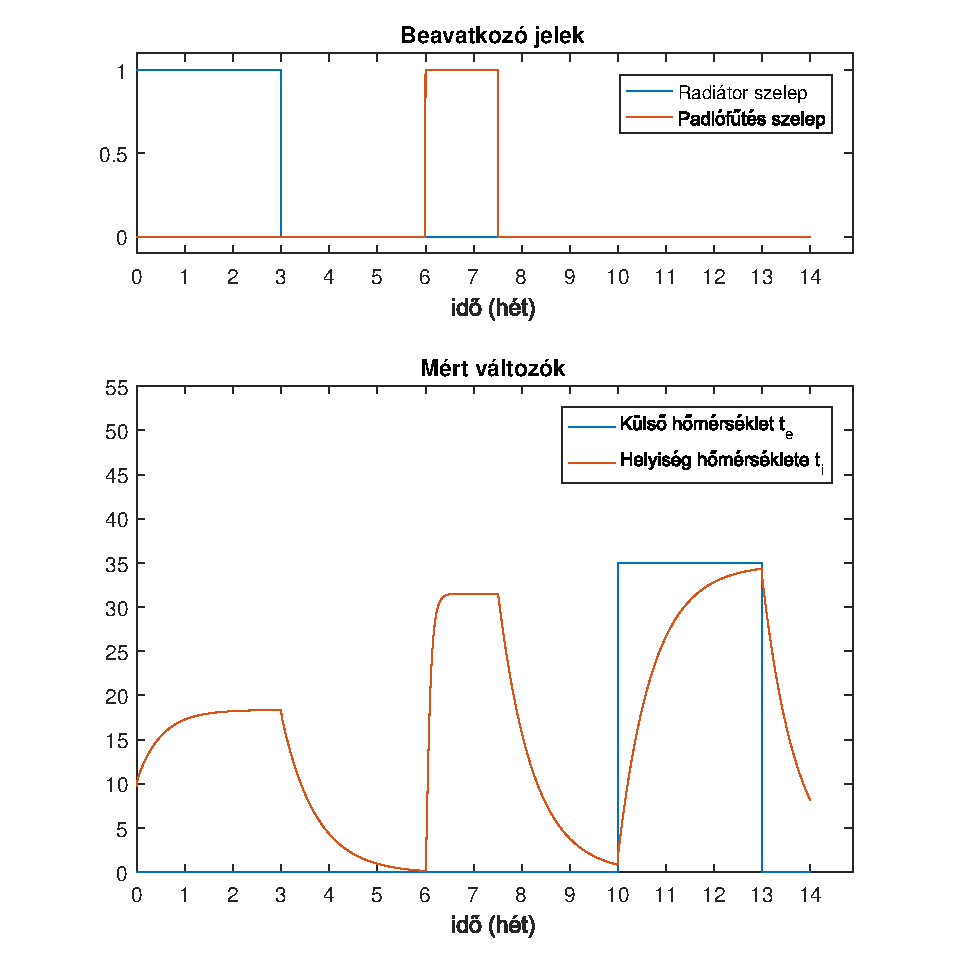
\includegraphics[trim=0 0 0 0, clip,width=0.7\textwidth]{figures/ident-valve2}
	\caption{Identifikáció során }
	\label{fig:ident}
\end{figure}

A módszer az, amit a több forrást tartalmazó hálózatok esetén is alkalmazunk: a válasz számításakor mindig egy forrás hatását vizsgáltuk, a többit dezaktivizáltuk: azaz a több bemenetű Simulink hálózatnak egyszerre csak egy bemenetét gerjesztem. Ez látható a felső ábrán. A kimeneten a válasz ekkor szuperpozícióval adódik. 

\textbf{ÁBRA: BEMENETEK ÉS AZOKRA ADOTT GERJESZTÉSEK}

A Simulink modellt bemenetein gerjesztem (külső hőmérséklet ablak \SI{40}{\celsius} 5 napig, majd fűtés \SI{60}{\celsius} előremenő hőmérsékleten valve = 1 állásban.\footnote{A stratégia lehet $t_s$ előremenő hőmérséklet vagy $\alpha \cdot \dot m$ tömegáram szabályzása $\alpha$ = [0..1] beavatkozójellel. })


Az identifikációhoz adatfile-t hozok létre, az IDDATA Simulink blokk rögzíti a be- és kimenetek értékét mintavételi időnként. A mintavételi idő először egy másodperc volt. A Matlab Workspace-ben megjelenik egy iddata, ezt tudom az ident toolboxba importálni. Erre átviteli függvényeket illesztek. Az átviteli függvények pólusainak, zérusainak a száma a Simscape modell alapján meghatározható, illetve intuícióból.

Nyilvánvalóan célszerű az identifikációnál minél nagyobb változásokat mérni. Nem tartottam "értelmét" 1\si{\celsius}-os step jelre identifikálni. Így beállítottam nulla kezdeti értéket a ház összes paraméterére. (Falak, fűtési rendszer, stb. Nyilvánvaló, hogy ilyenkor nem a realizmus a cél, hiszen a nagy változásokra jön elő a rendszer dinamikája.) Nulla kezdeti értékből a környezeti hőmérsékletet 0-ról 40\si{\celsius}-ra emeltem, ennek a beállási ideje több nap volt, majd visszaállítva 0\si{\celsius}-ra megvártam a lecsengést, ezután pedig a beavatkozó szelepeket teljesen kinyitottam. 

Egy ilyen szimuláció a fenti szekvenciával kb. 50 napnyi viselkedést fog át, ez másodperces mintavételi idővel rengeteg adat, amivel meggyűlik az Ident Toolbox baja is.

5 perces mintavételi időkkel már sokkal gyorsabban lefut a Simulinkben a szimuláció és a toolboxban az identifikáció, lénygében azonos eredményt adva. Az időállandók sokkal 

Viszont a mintavételi idők megváltoztatásától azért \textit{féltem}, mert nem tudtam, hogy reagál rá a Simscape vagy az MPC.

Zérusok hatása röviden. Mit tud. Hánytárolós rendszer. Néhány kép.
MISO identifikáció. 


\section{Hagyományos szabályzás performanciája}

PI, miért nem jó
Csak SISO-ra működik és itt esetünkben itt több bemenetről van szó mindenképpen. Irodalom: S. Prívara et al. 



\pagebreak